\documentclass{article}
\usepackage{tikz}
\usetikzlibrary{graphs, graphs.standard, quotes}

\begin{document}

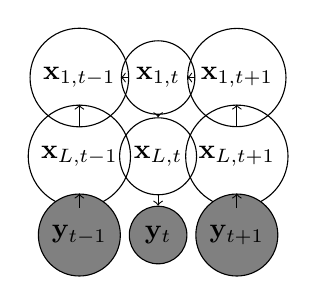
\begin{tikzpicture}[node distance=1cm]
    \node (x1t-1) [circle, draw] {$\mathbf{x}_{1,t-1}$};
    \node (x1t) [circle, draw, right of=x1t-1] {$\mathbf{x}_{1,t}$};
    \node (x1t+1) [circle, draw, right of=x1t] {$\mathbf{x}_{1,t+1}$};

    \node (xLt-1) [circle, draw, below of=x1t-1] {$\mathbf{x}_{L,t-1}$};
    \node (xLt) [circle, draw, below of=x1t] {$\mathbf{x}_{L,t}$};
    \node (xLt+1) [circle, draw, below of=x1t+1] {$\mathbf{x}_{L,t+1}$};

    \node (yt-1) [circle, draw, fill=gray, below of=xLt-1] {$\mathbf{y}_{t-1}$};
    \node (yt) [circle, draw, fill=gray, below of=xLt] {$\mathbf{y}_{t}$};
    \node (yt+1) [circle, draw, fill=gray, below of=xLt+1] {$\mathbf{y}_{t+1}$};

    \draw[->] (x1t-1) -- (x1t);
    \draw[->] (x1t) -- (x1t+1);

    \draw[->] (x1t-1) -- (xLt-1);
    \draw[->] (x1t) -- (xLt);
    \draw[->] (x1t+1) -- (xLt+1);

    \draw[->] (xLt-1) -- (yt-1);
    \draw[->] (xLt) -- (yt);
    \draw[->] (xLt+1) -- (yt+1);
\end{tikzpicture}

\end{document}